\documentclass[
	a4paper,
	oneside,
	BCOR = 10mm,
	DIV = 12,
	12pt,
	headings = normal,
]{scrartcl}

%%% Length calculations
\usepackage{calc}
%%%

%%% Support for color
\usepackage{xcolor}
\definecolor{lightblue}{HTML}{03A9F4}
\definecolor{red}{HTML}{F44336}
%%%

%%% Including graphics
\usepackage{graphicx}
%%%

%%% Font selection
\usepackage{fontspec}

\setromanfont{STIX Two Text}[
	SmallCapsFeatures = {LetterSpace = 8},
]

\setsansfont{IBM Plex Sans}[
	Scale = MatchUppercase,
]

\setmonofont{IBM Plex Mono}[
	Scale = MatchUppercase,
]
%%%

%%% Math typesetting
\usepackage{amsmath}

\usepackage{unicode-math}
\setmathfont{STIX Two Math}

\usepackage{IEEEtrantools}
%%%

%%% List settings
\usepackage{enumitem}
\setlist[enumerate]{%
	label*      = {\arabic*.},
	leftmargin  = *,
	labelindent = \parindent,
	topsep      = 1\baselineskip,
	parsep      = 0\baselineskip,
	itemsep     = 1\baselineskip,
	noitemsep, % override itemsep
}

\setlist[itemize]{%
	label*      = {—},
	leftmargin  = *,
	labelindent = \parindent,
	topsep      = 1\baselineskip,
	parsep      = 0\baselineskip,
	itemsep     = 1\baselineskip,
	noitemsep, % override itemsep
}

\setlist[description]{%
	font        = {\rmfamily\upshape\bfseries},
	topsep      = 1\baselineskip,
	parsep      = 0\baselineskip,
	itemsep     = 0\baselineskip,
}

%%%

%%% Structural elements typesetting
\setkomafont{pagenumber}{\rmfamily\upshape}
\setkomafont{disposition}{\rmfamily\bfseries}

% Sectioning
\RedeclareSectionCommand[
	beforeskip = -1\baselineskip,
	afterskip  = 1\baselineskip,
	font       = {\normalsize\bfseries\scshape},
]{section}

\RedeclareSectionCommand[
	beforeskip = -1\baselineskip,
	afterskip  = 1\baselineskip,
	font       = {\normalsize\bfseries\itshape},
]{subsection}

\RedeclareSectionCommand[
	beforeskip = -1\baselineskip,
	afterskip  = 1\baselineskip,
	font       = {\normalsize\bfseries},
]{subsubsection}

\RedeclareSectionCommand[
	beforeskip = -1\baselineskip,
	afterskip  = -0.5em,
	font       = {\normalsize\mdseries\scshape\addfontfeatures{Letters = {UppercaseSmallCaps}}},
]{paragraph}
%%%

%%% Typographic enhancements
\usepackage{microtype}
%%%

%%% Language-specific settings
\usepackage{polyglossia}
\setmainlanguage{ukrainian}
\setotherlanguages{english}
%%%

%%% Captions
\usepackage{caption}
\usepackage{subcaption}

%\DeclareCaptionLabelFormat{closing}{#2)}
%\captionsetup[subtable]{labelformat = closing}

%\captionsetup[subfigure]{labelformat = closing}

\captionsetup[table]{%
	aboveskip = 0\baselineskip,
	belowskip = 0\baselineskip,
}

\captionsetup[figure]{%
	aboveskip = 1\baselineskip,
	belowskip = 0\baselineskip,
}

\captionsetup[subfigure]{%
	labelformat = simple,
	labelformat = brace,
}
%%%

%%% Hyphenated ragged typesetting
\usepackage{ragged2e}
%%%

%%% Table typesetting
\usepackage{booktabs}
\usepackage{longtable}

\usepackage{multirow}

\usepackage{array}
\newcolumntype{v}[1]{>{\RaggedRight\arraybackslash\hspace{0pt}}p{#1}}
\newcolumntype{b}[1]{>{\Centering\arraybackslash\hspace{0pt}}p{#1}}
\newcolumntype{n}[1]{>{\RaggedLeft\arraybackslash\hspace{0pt}}p{#1}}
%%%

%%% Drawing
\usepackage{tikz}
\usepackage{tikzscale}
\usetikzlibrary{arrows.meta} % Stealth arrow tips
\usetikzlibrary{positioning}
\usetikzlibrary{shapes.geometric} % Stealth arrow tips
%%%

%%% SI units typesetting
\usepackage{siunitx}
\sisetup{%
	output-decimal-marker = {,},
	exponent-product      = {\cdot},
	inter-unit-product    = \ensuremath{{} \cdot {}},
	per-mode              = symbol,
}
%%%

%%% Framing code listings
\usepackage{tcolorbox}
\tcbuselibrary{breakable}
\tcbuselibrary{minted}
\tcbuselibrary{skins}

\newtcblisting[
	auto counter,
	list inside,
	number within = section,
]{listingpython}[3][]{%
	minted language = python,
	minted style    = bw,
	minted options  = {%
		linenos,
		tabsize = 4,
		breaklines,
		% breakanywhere,
		fontsize = \footnotesize,
		autogobble
	},
	%
	% empty,
	sharp corners,
	colframe         = black,
	colback          = black!0,
	leftrule         = 0em,
	rightrule        = 0em,
	toprule          = 1pt, % orig = 0pt
	bottomrule       = 1pt, % orig = 0pt
	titlerule        = 0.5pt,
	colbacktitle     = black!0,
	coltitle         = black,
	toptitle         = 0.3em,
	bottomtitle      = 0.1em,
	borderline north = {1pt}{0pt}{black},
	borderline south = {1pt}{0pt}{black},
	before skip      = \intextsep,
	after  skip      = \intextsep,
	title            = {Лістинг \thetcbcounter: #2},
	list entry       = {\protect\numberline{\thetcbcounter}#2},
	left = 0em,
	right = 0em,
	%
	listing only,
	breakable,
	%
	label = {#3},
	%
	#1
}

\newtcbinputlisting[auto counter, list inside, number within = section]{\inputpython}[4][]{%
	minted language = python,
	minted style    = bw,
	minted options  = {%
		linenos,
		tabsize = 4,
		breaklines,
		breakbytokenanywhere,
		fontsize = \footnotesize,
	},
	%
	% empty,
	sharp corners,
	colframe         = black,
	colback          = black!0,
	leftrule         = 0em,
	rightrule        = 0em,
	toprule          = 0pt, % orig = 0pt
	bottomrule       = 0pt, % orig = 0pt
	titlerule        = 0.5pt,
	colbacktitle     = black!0,
	coltitle         = black,
	toptitle         = 0.3em,
	bottomtitle      = 0.1em,
	borderline north = {1pt}{0pt}{black},
	borderline south = {1pt}{0pt}{black},
	before skip      = \intextsep,
	after  skip      = \intextsep,
	title            = {Лістинг \thetcbcounter: #3},
	list entry       = {\protect\numberline{\thetcbcounter}#3},
	left = 0em,
	right = 0em,
	%
	listing file={#2},
	listing only,
	breakable,
	%
	label = {#4},
	%
	#1
}

% Customize minted
\usepackage{minted}
\setmintedinline{%
	style = bw,
	breaklines,
}

% Customize minted line numbers
\renewcommand{\theFancyVerbLine}{\ttfamily\scriptsize\arabic{FancyVerbLine}}

%%%

%%% Sideways table
\usepackage{pdflscape}
%%%

%%% Wrap text after sideways table
\usepackage{afterpage}
%%%

%%% Links and hyperreferences
\usepackage{hyperref}
\hypersetup{%
	bookmarksnumbered = true,
	colorlinks      = false,
	linkbordercolor = red,
	urlbordercolor  = lightblue,
	pdfborderstyle  = {/S/U/W 1.5},
}
%%%

%%% Length adjustments
% Set baselineskip, default is 14.5 pt
\linespread{1.068966} % ~15.5 pt
\setlength{\emergencystretch}{1em}
\setlength{\parindent}{1.5em}
\newlength{\gridunitwidth}
\setlength{\gridunitwidth}{\textwidth / 12}
%%%

%%% Custom commands
\newcommand{\allcaps}[1]{{\addfontfeatures{LetterSpace = 8, Kerning = Off}#1}}
\newcommand{\filename}[1]{\texttt{#1}}
\newcommand{\progname}[1]{\texttt{#1}}
\newcommand{\modulename}[1]{\texttt{#1}}
%%%

%%% Custom math commands
\newcommand{\longvar}[1]{\mathit{#1}}
%%%

\begin{document}

\begin{titlepage}
		\begin{center}
			Міністерство освіти і~науки України\\
			Національний авіаційний університет\\
			Навчально-науковий інститут комп'\-ютерних інформаційних технологій\\
			Кафедра комп'\-ютеризованих систем управління

			\vspace{\fill}
				Лабораторна робота №5\\
				з~дисципліни «Комп'\-ютерні системи»\\
				на~тему «Архітектура конвеєрних обчислювальних систем»\\
				Варіант~№8

			\vspace{\fill}

			\begin{flushright}
				Виконав:\\
				студент \allcaps{ННІКІТ}\\
				групи СП-325\\
				Клокун В.\,Д.\\
				Перевірив:\\
				Ковальов М.\,О.
			\end{flushright}

			Київ 2019
		\end{center}
	\end{titlepage}

	\section{Мета роботи}
		Аналіз структур конвеєрних обчислювальних систем.

	\section{Загальні теоретичні відомості}

	\section{Хід роботи}
		Вихідними даними для лабораторної роботи є~арифметичний вираз. Для варіанту~№~8 він виглядає так:
		\begin{IEEEeqnarray}{rCl}
			A \div B + (C + D \times E) \times (G + K \div L \times M).
		\end{IEEEeqnarray}
		За даним виразом складаємо дерево арифметичного виразу~(рис.~\ref{fig:expression-tree}).

		\begin{figure}[!htbp]
			\centering
			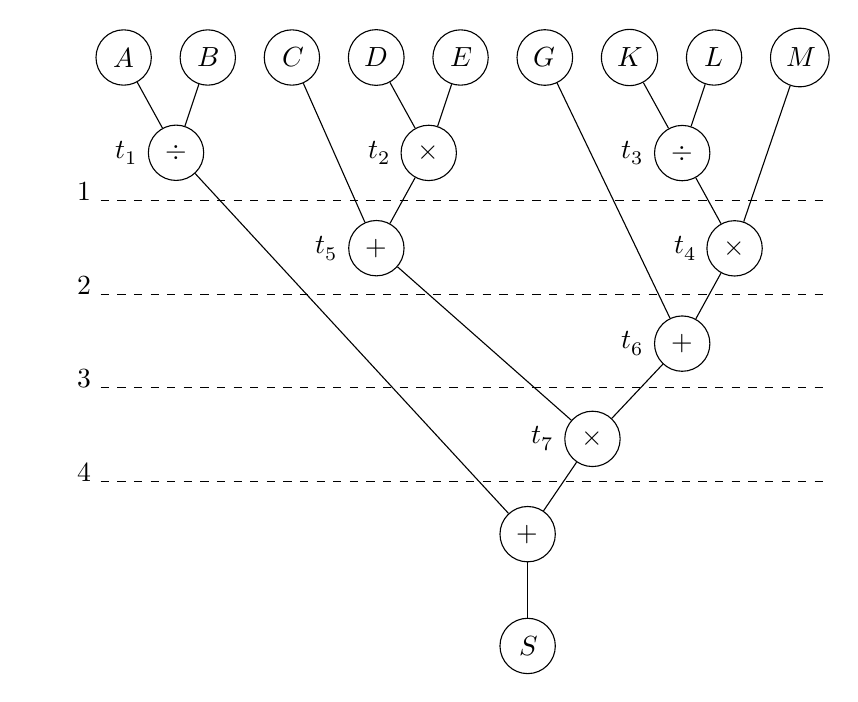
\begin{tikzpicture}[]
				\tikzset{main node/.style={circle,draw,minimum size=2em}}
				\tikzset{every label/.style={label position=left}}
				\node[main node] (l05-a) {$A$};
				\node[main node, right = 1em of l05-a] (l05-b) {$B$};
				\node[main node, right = 1em of l05-b] (l05-c) {$C$};
				\node[main node, right = 1em of l05-c] (l05-d) {$D$};
				\node[main node, right = 1em of l05-d] (l05-e) {$E$};
				\node[main node, right = 1em of l05-e] (l05-g) {$G$};
				\node[main node, right = 1em of l05-g] (l05-k) {$K$};
				\node[main node, right = 1em of l05-k] (l05-l) {$L$};
				\node[main node, right = 1em of l05-l] (l05-m) {$M$};

				\node[main node, label={$t_1$}, below right = 2em and 0.45em of l05-a]  (l04-div-01) {$\div$};
				\node[main node, label={$t_2$}, below right = 2em and 0.45em of l05-d]  (l04-mul-01) {$\times$};
				\node[main node, label={$t_3$}, below right = 2em and 0.45em of l05-k]  (l04-div-02) {$\div$};

				\node[main node, label={$t_5$}, below left  = 2em and 0.45em of l04-mul-01]  (l03-plus-01) {$+$};
				\node[main node, label={$t_4$}, below right = 2em and 0.45em of l04-div-02]  (l03-mul-01) {$\times$};

				\node[main node, label={$t_6$}, below left  = 2em and 0.45em of l03-mul-01] (l02-plus-01) {$+$};

				\node[main node, label={$t_7$}, below left  = 2em and 1.80em of l02-plus-01] (l01-mul-01) {$\times$};

				\node[main node, below left  = 2em and 0.9em of l01-mul-01] (root-plus) {$+$};

				\node[main node, below = 2em of root-plus] (root-S) {$S$};

				\path[draw]
				(root-S)     edge node {} (root-plus)
				(root-plus)  edge node {} (l01-mul-01)
				             edge node {} (l04-div-01)
				(l01-mul-01) edge node {} (l02-plus-01)
				             edge node {} (l03-plus-01)
				(l02-plus-01) edge node {} (l03-mul-01)
				              edge node {} (l05-g)
				(l03-mul-01)  edge node {} (l04-div-02)
				              edge node {} (l05-m)
				(l03-plus-01) edge node {} (l04-mul-01)
				              edge node {} (l05-c)
				(l04-div-01) edge node {} (l05-a)
				             edge node {} (l05-b)
				(l04-mul-01) edge node {} (l05-d)
				             edge node {} (l05-e)
				(l04-div-02) edge node {} (l05-k)
				             edge node {} (l05-l)
				;

				%\path[dashed] (current bounding box.west) -- (current bounding box.east);
				\node [below left = 0em and 2em of l04-div-01] (l04) {Ярус 1};
				\node [below = 2em of l04] (l03) {Ярус 2};
				\node [below = 2em of l03] (l02) {Ярус 3};
				\node [below = 2em of l02] (l01) {Ярус 4};

				\draw [dashed] (l04.base east) -- (l04.base east -| l05-m.east);
				\draw [dashed] (l03.base east) -- (l03.base east -| l05-m.east);
				\draw [dashed] (l02.base east) -- (l02.base east -| l05-m.east);
				\draw [dashed] (l01.base east) -- (l01.base east -| l05-m.east);

			\end{tikzpicture}
			\caption{Дерево арифметичного виразу $A \div B + (C + D \times E) \times (G + K \div L \times M)$}
			\label{fig:expression-tree}
		\end{figure}

	\section{Висновок}
		Виконуючи дану лабораторну роботу, ми~проаналізували структури конвеєрних обчислювальних систем.

\end{document}

